
\chapter{Materials and Methods}

\section{Instruments and Apparatus}

The experiment described requires a number of computer systems and associated
hardware to run the simulation and capture appropriate data. This equipment is
described in the following chapter.

\subsection{Hub/Managed Router}

The network equipment chosen to run the experiment is a simple hub or
'repeater' which duplicates all packets transmitted on all ports. This makes it
easy to monitor all communications across the network for analysis purposes
\parencite{website:hub-reference}.

\subsection{Tor Software}


\subsection{'tcpdump' Software}

The tcpdump software captures network packets that are transferred using
network interfaces attached to the current hardware \parencite{:2009cr}.  It is
available on most operating systems and supports a flexible filtering language
for capturing only the specific packets desired. The format of output produced
by tcpdump is well documented \parencite{:nx} which makes it ideal for
transformation and processing by third party tools.

\subsection{Weka Software}

Weka is data mining software which includes tools for classification of data
sources using a wide variety of machine learning algorithms
\parencite{Hall:2009p7662}.

\subsection{VirtualBox Software}

VirtualBox is virtualization software that allows the running of a guest
operating system in its own environment on another host operating system
\parencite{:fk}.  It supports snapshots and a remote control facility which
make it useful for running repetitions in an experimental environment
\parencite{:uq}.

\subsection{Ruby Software}

Ruby is an object orientated, dynamic programming language which is useful for
quick prototyping and as such has been used to automate the simulation
described in this experiment \parencite{:2010uq}.

(I used it because it is a language that is fast to develop in and I am
familiar with it)

\subsection{Ubuntu Linux Software}

The Ubuntu Linux operating system is freely available Linux operating system
available for desktop personal computers.

\cite{:2010ly}

\subsection{Selenium Software}

Selenium is a web testing framework with a number of components that allow
developers to write automated tests of web applications using most modern web
browsers \parencite{:2010ys}. Using the Selenium framework one can mimic the
actions of an actual user interacting with a web site.

\subsection{Firefox Software}

Firefox is a web browser developed by the Mozilla organization and freely
available for most desktop personal computers \parencite{mozilla}. It's strong
standards compliance \parencite{Hammond:2010fk} and popularity
\parencite{:2010kx,:2010vn} on the simulation platform make it an ideal
candidate for this experiment.

\subsection{OpenSSH Software}

OpenSSH is a freely available suite of connectivity tools
\parencite{:2010zr,:ve} that supports remote command execution
\parencite{Tucker:2010ly}.

\cite{:2010zr}

\subsection{Apache Software}

The Apache web server is the most prevalent web server used on the internet
\parencite{2010:dq}.  \cite{:qf}

\subsection{Sinatra Software}

Sinatra is a simple framework for creating dynamic web applications using the
Ruby programming language \parencite{:2010bh}.

\section{Procedure}

The experiment involves two stages, an initial configuration stage to prepare
equipment, install software, configure and test the design and the final stage
of executing the simulation to capture packet traces.

\subsection{Hardware Configuration}

Four identical IBM desktop computer systems were prepared and arranged as shown
in figure \ref{physical-setup}.

\begin{figure}[H]
  \centering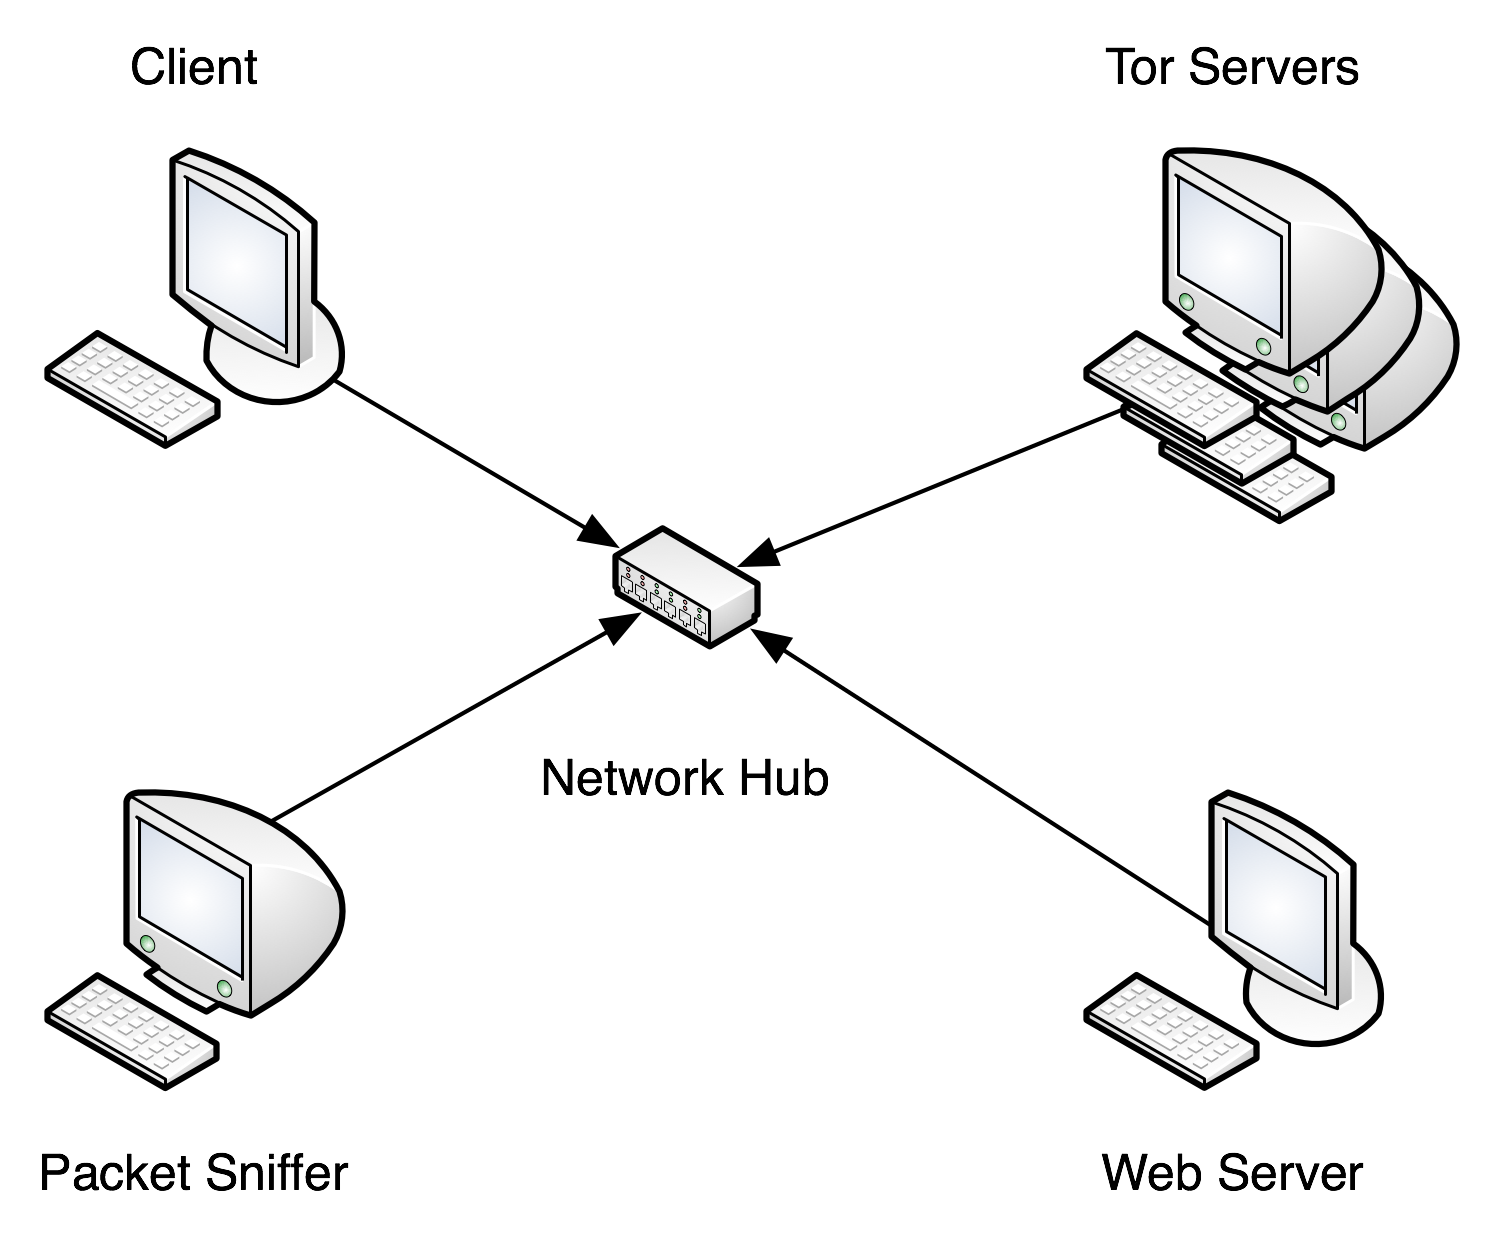
\includegraphics[scale=0.7]{physical-setup}
  \caption{Physical Setup}
  \label{physical-setup}
\end{figure}

\subsection{Software Configuration}

Table \ref{table:hosts} shows the role of each system in the experiment as well
as the edition of operating system in use and the IP address they were
configured with on the network.

\begin{tabular}{lrr}
  \toprule
  Role & Operating System Version & IP Address\\
  \midrule
  Client Host & Desktop & 192.168.0.100\\
  Server Host & Desktop & 192.168.0.001\\
  Tor Host & Desktop & 192.168.0.102\\
  \midrule
  Sniffing System & Server & 192.168.0.200\\
  \midrule
  Client Guest & Desktop & 192.168.0.16\\
  Server Guest & Server & 192.168.0.17\\
  Tor Network Guest & Server & 192.168.0.18\\
  \botomrule
  \label{table:hosts}
\end{tabular}

Figure \ref{network-diagram} shows the placement of applications and relevant
data flows.

\begin{figure}[H]
  \centering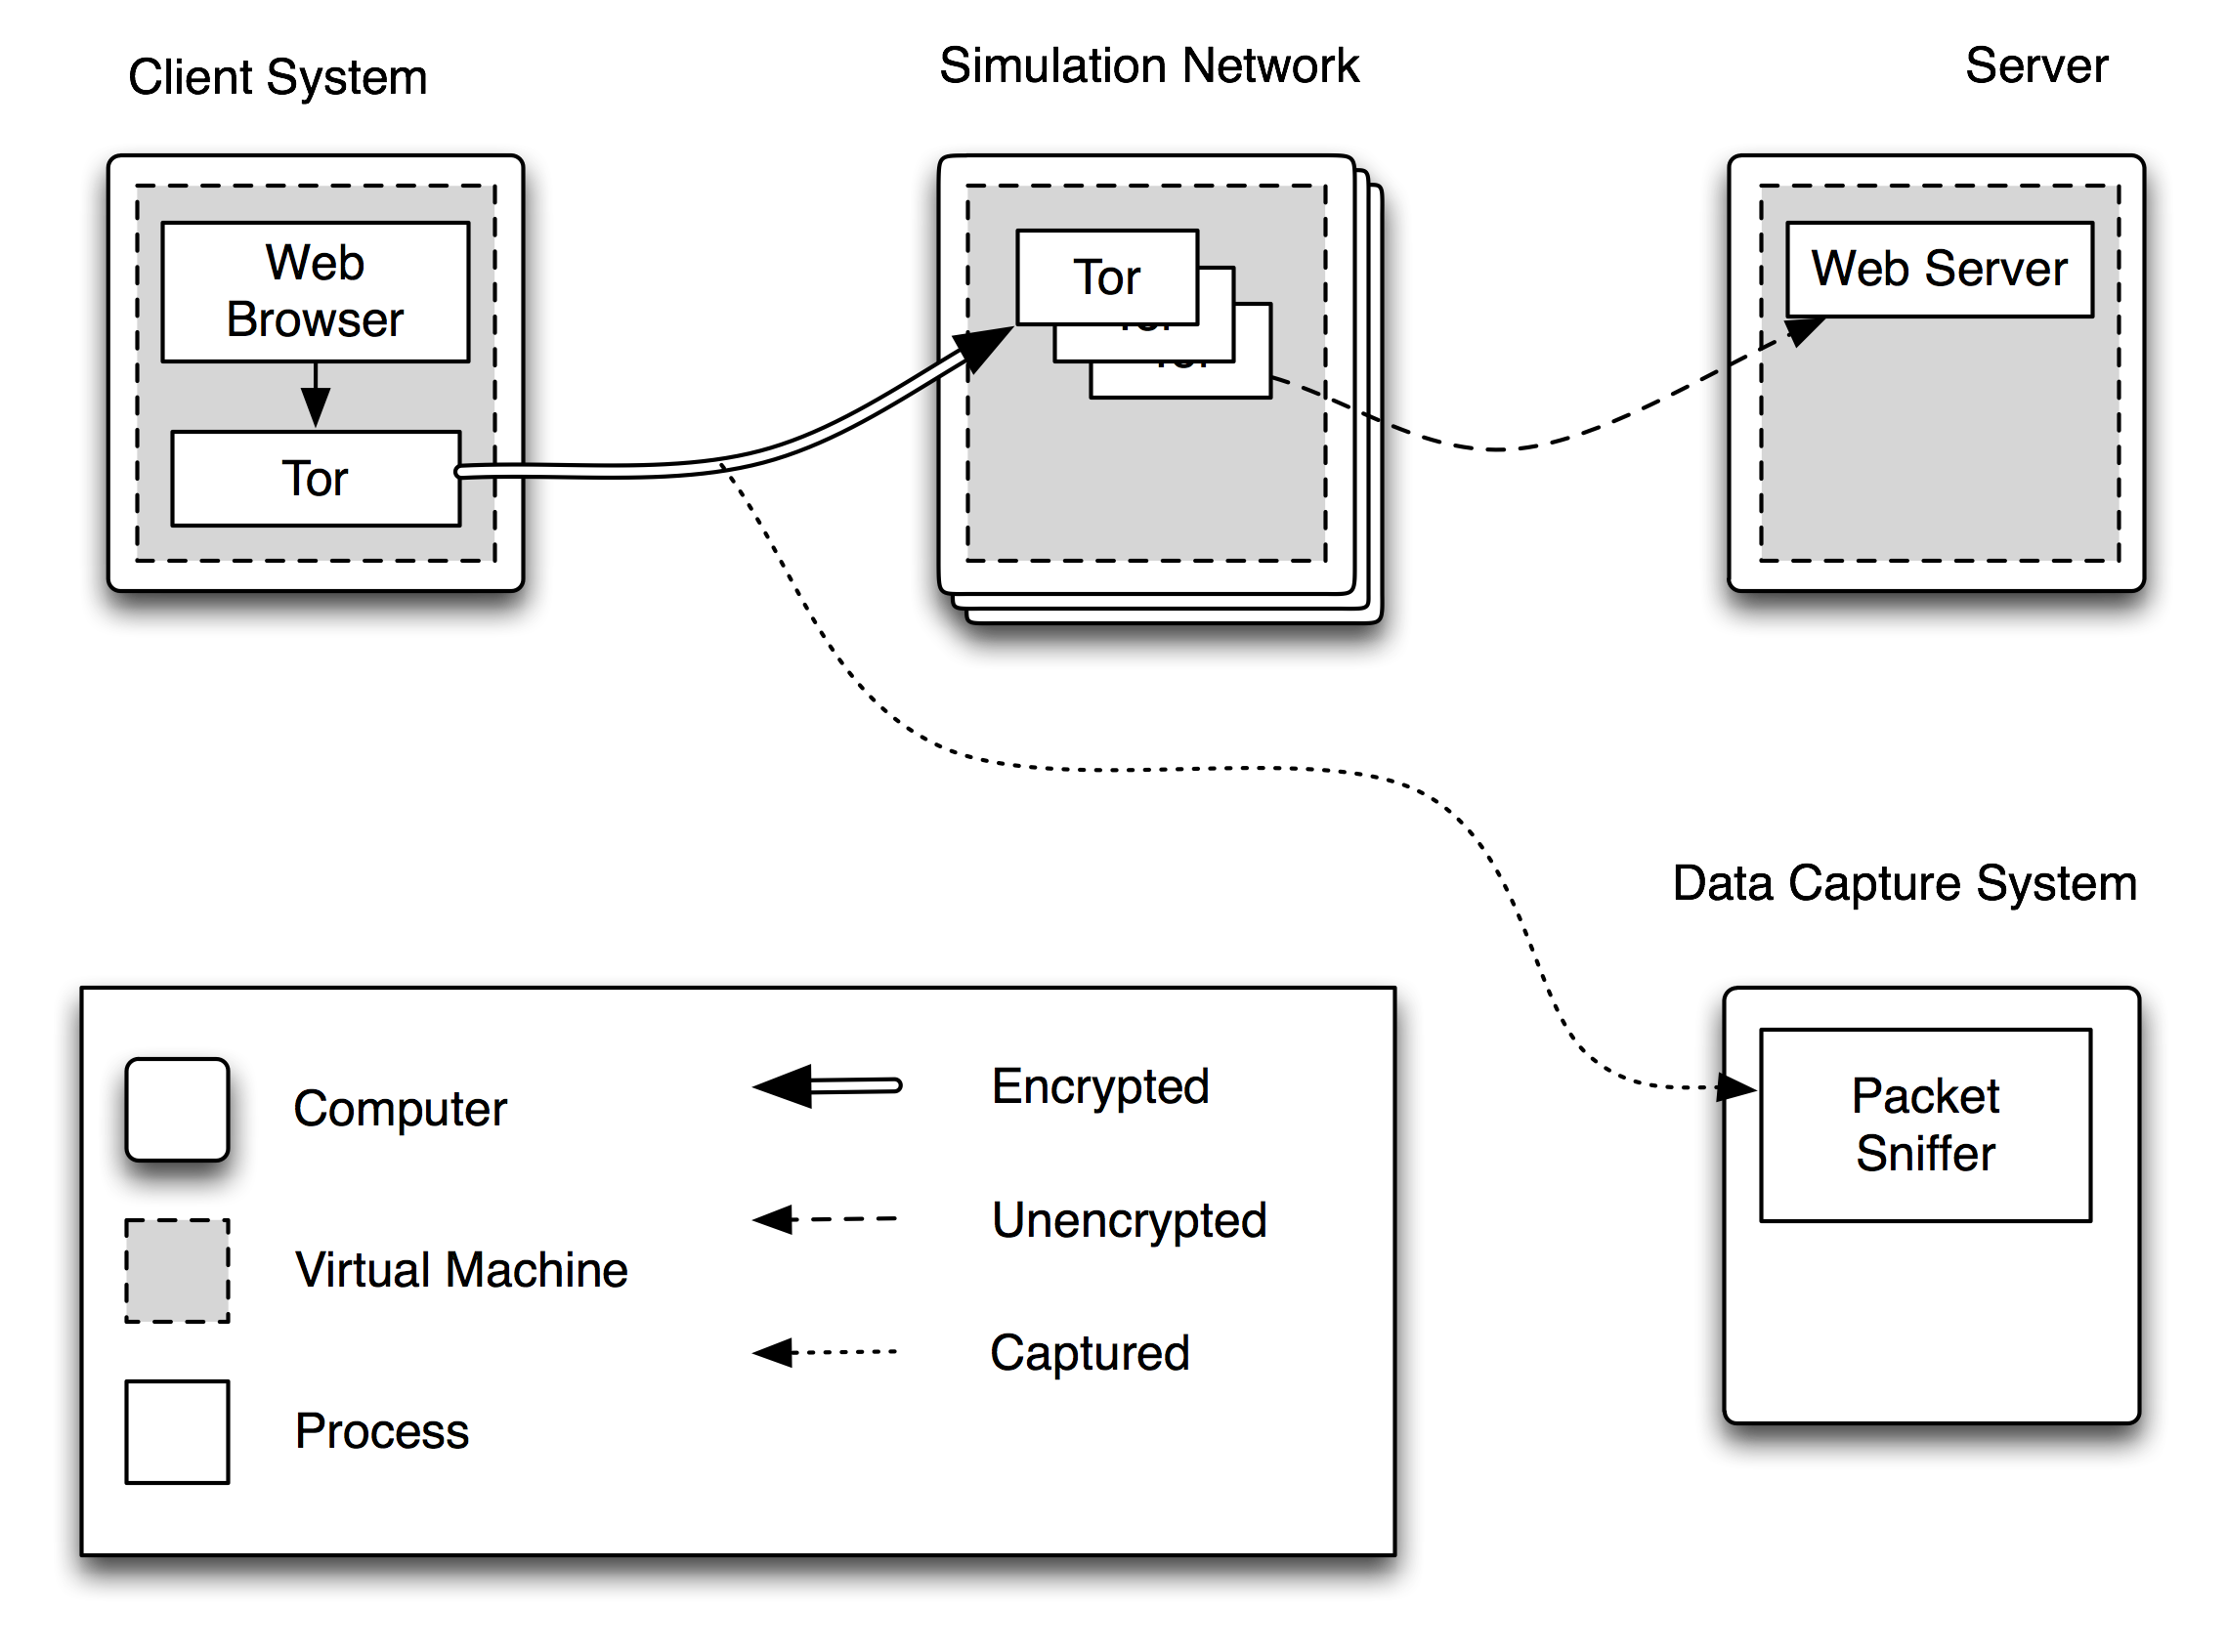
\includegraphics[width=\linewidth]{network-diagram}
  \caption{Network Diagram}
  \label{network-diagram}
\end{figure}

\subsection{Sniffing System}

The sniffing system was based on a basic installation of the Ubuntu 10.04 server
operating system with no additional packages installed.

An init.d script was installed to execute the tcpdump program with a specific
filter string after the system had powered on. All capture files were limited to
1mb in size and put into a time stamped directory. To ensure that only relevant
packets were collected the filter string was tuned for each phase of the
experiment. The filter string for each phase is shown below.

Phase 1:
\begin{lstlisting}[language=sh]
dst port 443
\end{lstlisting}

Phase 2 and 3:
\begin{lstlisting}[language=sh]
dst port 5000-5015
\end{lstlisting}

\subsection{Host Systems}

All the host systems are configured identically. The following procedure is
carried out to prepare a host system.

\begin{itemize*}
  \item Install Ubuntu 10.04 Desktop Operating System
    \begin{itemize*}
      \item Use entire disk
      \item Set time zone to GMT +8 WST (Perth)
    \end{itemize*}
  \item Turn off automatic package updates
  \item Turn off power saving features
  \item Install OpenSSH Server
  \item Add Virtual Box repository to sources.lst
  \item Update sources and install Virtual Box
  \item Ensure Virtual Box starts with system and disable all other start
    up applications
\end{itemize*}

One of the host systems is set aside as a management system, which is
responsible for ensuring the experiment runs and restarts it if there are any
problems. On this machine a private ssh key is created, and copied to the
authorized keys file on all other hosts. This allows the management system to
connect to all the other systems and issue commands without user interaction.

The management script runs on the management system to watch the experiment's
progress. This is a simple Ruby script which uses SSH to control the other Host
systems and opens a socket which waits for a connection that indicates that the
experiment has finished. Every time it starts the experiment, it rolls back
each virtual machine to a preconfigured snapshot. If the experiment takes too
long, say because a virtual machine hangs or something is wrong, it will be
started without waiting for the finish condition.

Note that restarting each snapshot ensures that the system clock of each guest
operating system is synchronized with that of the host operating system. The
Tor network is sensitive to differences in time between hosts and this ensures
correct operation.

\subsection{Guest Systems}

\subsubsection{Client System}

The client system runs Ubuntu 10.04 Desktop Operating System as well as a
number of applications that allow it to perform automated web browsing. Tor is
configured on this system as well for the Tor part of the experiment but is
initially disabled.

The software installed on this system includes:

\begin{itemize*}
  \item Ruby
  \item Rubygems:
    \begin{itemize*}
      \item Selenium
      \item DaemonController
      \item RSpec
    \end{itemize*}
  \item Selenium-RC
  \item Firefox web browser
  \item Tor
\end{itemize*}

The client operation is controlled by a Ruby script which ensures that the
Selenium-RC server is running, executes a number of Selenium browser
simulations using RSpec and reports it's success by connecting to an open
socket on the management system.

There are 170 simulations which emulate simple website interactions which have
different traffic profiles against 30 different websites on the Server system.

For the non-SSL portion of the experiment, Selenium is configured to use a
special proxy which automatically accepts self signed certificates. Typical
interactions with SSL encrypted websites are signed by a certificate authority,
so no user interaction is required to begin browsing.

\subsubsubsection{Selenium}

SSL + Tor over selenium. 

Generate a selenium firefox profile. First launch selenium in interactive mode specifying a proxy:

\begin{lstlisting}[language=sh]
java -jar $selenium.jar -interactive
\end{lstlisting}

This will start a prompt to which you can edit commands, you must launch a browser to get selenium to create a firefox profile directory.

cmd=getNewBrowserSession&1=*firefoxproxy&2=http://www.google.com

Generate a firefox profile, then edit the proxy.pac file to 

\begin{lstlisting}[language=sh]
function FindProxyForURL(url, host) {
   if(shExpMatch(url, '*/selenium-server/*')) {
       return 'PROXY localhost:4444; PROXY proxy.ourdomain.dom:8080';
   } else if (shExpMatch(host, '*dev.ourdomain.dom*')) {
       return 'DIRECT';
   } else if (shExpMatch(host, '*qa.ourdomain.dom*')) {
       return 'DIRECT';
   } else if (shExpMatch(host, '*staging.ourdomain.dom*')) {
       return 'DIRECT';
   } else {
       return 'PROXY proxy.ourdomain.dom:8080';
   }
}
\end{lstlisting}

or

\begin{lstlisting}[language=sh]
function FindProxyForURL(url, host) {
   if(shExpMatch(host, '*torsim')) {
       return 'PROXY localhost:8118';
   }
   return 'PROXY localhost:4444; DIRECT';
}
\end{lstlisting}

This makes sure that your proxy (Tor) gets used for outgoing connections, and the selenium proxy is used for running tests.

To get SSL certificates accepted, you must manually accept them permanently for each host. This will update the cert_override.txt and cert8.db files.

Tor must have the following setting supplied:

\begin{lstlisting}[language=sh]
ExitPolicyRejectPrivate 0
\end{lstlisting}

Since we are using a 192.* network. - Not true, testing mode flag sets this.

But the tor relays must be able to resolve names using DNS, if you use socks4a protocol.

\subsubsection{Server System}

The host system runs an apache web server which serves two sets of sample
websites, static and dynamic. The static websites are served each from a
different numbered directory and accessible over a different virtual host. This
means that when a web browser is pointed at the directory
\verb+site1.static.torsim+ the files in
\verb+/var/www/thesis/experiment/simulation/static/site1+ are served to the
browser.

For the SSL part of the experiment, only the HTTPS port 443 is accessed and all
information is sent to the browser using encryption.

The dynamic sample websites change subtly with each attempted access. There are
10 sample websites each a slightly different Ruby Sinatra application.

\subsubsection{Tor Simulation}

The Tor Simulation Guest is responsible for emulating a Tor network. It runs
three Tor directory authorities as well as fifteen relays.

Each Tor instance on the Tor Simulation system is given it's own separate
directory for configuration, logging and temporary files.

\section{Procedure}

\subsection{Preparation}

\subsubsection{Host Systems}

The preparation for the host operating systems is identical except for the
hostname and IP address.

Installing the Host operating system:

\begin{enumerate*}
  \item Power on machine
  \item Interrupt BIOS boot process
  \begin{enumerate*}
    \item Load default BIOS settings
    \item Set boot order to ensure CD-ROM is first
    \item Disable unnecessary boot devices
    \item Ensure system clock is correct
  \end{enumerate*}
  \item Boot from Ubuntu 10.04 Desktop cd
  \item Select the language you wish to use for installation (English) and click 'Forward'
  \item Select the region (Australia/Perth) and click 'Forward'
  \item Select an appropriate keymap (USA) and click 'Forward'
  \item Select 'Erase and use the entire disk' and click 'Forward'
  \item Enter your details, select 'Log in automatically' and click 'Forward'
\end{enumerate*}

At this point the installation will begin and should take about 35 minutes.
'Log in automatically' is selected to ensure that the experiment will continue
even if power is lost. Once installation is complete remove the CD and reboot
the system.

Configuring the Host operating system:

\begin{enumerate*}
  \item Configure the network adapter
  \item Install Virtual Box
  \item Load the guest operating system virtual machine image
\end{enumerate*}

To install Virtual Box, the following procedure is used:

\begin{enumerate*}
  \item Edit the file \verb+/etc/apt/sources.lst+ and add the line:
  \begin{verbatim}
deb http://download.virtualbox.org/virtualbox/debian lucid non-free
  \end{verbatim}
  \item Install the GPG key for the Virtual Box packages:
  \begin{verbatim}
wget -q http://download.virtualbox.org/virtualbox/debian/oracle_vbox.asc -O- | sudo apt-key add -
  \end{verbatim}
  \item Then install VirtualBox 3.2 with the command:
  \begin{verbatim}
sudo apt-get update && sudo apt-get install virtualbox-3.2
  \end{verbatim}
\end{enumerate*}

For the management system, some additional commands need to be run:

\begin{enumerate*}
  \item Generate a private ssh key for the user with the command:
    \verb+ssh-keygen+, when prompted for a password enter nothing.
  \item SSH to the other host systems on the network, and copy the contents of
    \verb+$HOME/.ssh/id_rsa.pub+ into \verb+$HOME/.ssh/authorized_keys+ on the
    destination system.
  \item Install ruby so that the management script can be run:
    \begin{lstlisting}[language=sh]
sudo apt-get install ruby rubygems
    \end{lstlisting}
  \item Ensure the script \verb+run_simulation.rb+ is started on login.
\end{enumerate*}

\subsubsection{Tor System}

Install Ubuntu 10.04 Server.

Deploy the experiment files.

Install Tor:

\begin{enumerate*}
  \item Edit the file \verb+/etc/apt/sources.lst+ and add the line:
    \begin{lstlisting}[language=sh]
deb http://deb.torproject.org/torproject.org lucid main
    \end{lstlisting}
  \item Install the GPG key for the Tor packages:
    \begin{lstlisting}[language=sh]
gpg --keyserver keys.gnupg.net --recv 886DDD89
gpg --export A3C4F0F979CAA22CDBA8F512EE8CBC9E886DDD89 | sudo apt-key add -
    \end{lstlisting}
  \item Install Tor:
    \begin{lstlisting}[language=sh]
sudo apt-get update && sudo apt-get install tor
    \end{lstlisting}
\end{enumerate*}

\subsubsection{Client System}

Install Ubuntu 10.04 Desktop as in the Host system directions, leaving out the
Virtual Box installation.

\begin{enumerate*}
  \item Deploy the experiment files onto the client system.
  \item Install Ruby
  \item Install the bundler ruby gem with the command:
    \begin{lstlisting}[language=sh]
gem install bundler
    \end{lstlisting}
  \item Install the required client ruby gems by executing the bundler from the client directory in the deployed experiment files.
    \begin{lstlisting}[language=sh]
bundle install
    \end{lstlisting}
  \item Ensure that the client script is executed at system startup.
\end{enumerate*}

\subsubsection{Configuring the Management Script}

Once all systems are deployed, the management script needs to be altered to

\subsection{Execution}

Running the experiment is a matter of ensuring all Host systems are powered on,
if everything is configured correctly the experiment will continue to run until
stopped manually.

\subsection{Processing of Results}

The experiment was run over the course of 8 weeks yielding three sets of sample
data.

\begin{tabular}{lrr}
  \toprule
  Phase & Size (bytes) & Number of sessions\\
  \midrule
  HTTPS & 2326328 & 236659\\
  HTTP over Tor & 2869624 & 168876\\
  HTTPS over Tor & 1591112 & 95203\\
  \bottomrule
  \label{table:datasets}
\end{tabular}

The data captured was in the form of 1mb capture files which were recombined
with mergecap and processed by NetAI to produce ARFF format files for use by
Weka. Each data set were given the nominal classification 'http',
'http_over_tor' and 'https_over_tor', all other nominal attributes were removed.

% vim: fdm=syntax tw=80
